\documentclass[10pt,conference]{IEEEtran}
\IEEEoverridecommandlockouts

\usepackage{cite}
\usepackage{amsmath,amssymb,amsfonts}
\usepackage{algorithmic}
\usepackage{algorithm}
\usepackage{graphicx}
\usepackage{textcomp}
\usepackage{xcolor}
\usepackage{tabularx}
\usepackage{booktabs}
\usepackage{multirow}
\usepackage{hyperref}
\usepackage{listings}
\usepackage{pgfplots}
\pgfplotsset{compat=1.18}
\usepackage{float}

\def\BibTeX{{\rm B\kern-.05em{\sc i\kern-.025em b}\kern-.08em
    T\kern-.1667em\lower.7ex\hbox{E}\kern-.125emX}}

\begin{document}

\title{Multi-Depot Vehicle Routing Problem with Time Windows using Ant Colony Optimization: A Full-Stack Dashboard Approach}

\author{\IEEEauthorblockN{Sahil Kumar\textsuperscript{1}, [Member 2]\textsuperscript{2}, [Member 3]\textsuperscript{3}, [Member 4]\textsuperscript{4}}
\IEEEauthorblockA{\textit{Department of Computer Science \& Engineering} \\
\textit{[Institution Name]}\\
\textit{Faculty Guide: Prof. / Dr. [Faculty Name]}\\
India \\
Email: \{sahil, member2, member3, member4\}@institute.edu}
}

\maketitle

% ============================================================
% ABSTRACT
% ============================================================
\begin{abstract}
Efficient vehicle routing and load scheduling across multiple depots are critical for reducing operational logistics costs, minimizing total distance traveled, and ensuring strict adherence to delivery time constraints. This paper presents a comprehensive full-stack optimization framework for solving the Multi-Depot Vehicle Routing Problem with Time Windows (MDVRPTW). The proposed system employs a specialized Ant Colony Optimization (ACO) algorithm distributed across spatial K-Means partitioned clusters. A dynamic boundary adjustment strategy processes multi-objective transition probabilities to balance customer demands across multiple depots. The fitness evaluation integrates physical capacity limits and hard Solomon benchmark timeline bounds (ready and due times) via heavily penalized metrics. To prevent local optimization traps and algorithmic stagnation, the system continuously monitors the Shannon Entropy of the pheromone distribution grid, triggering evaporation and exploration bursts when diversity crashes are detected. A parallelized 2-opt intra-route local search acts as a hybrid refinement layer, yielding an additional 11--15\% distance reduction. Empirical validation across standardized Solomon datasets (C101, R101, RC101) alongside a high-fidelity geospatial React frontend mapping dashboard proves robust optimization stability. The framework exposes 15+ configurable hyperparameters through a functional web platform, providing real-time interpretability of the ACO routing logic to human planners.
\end{abstract}

\begin{IEEEkeywords}
MDVRP, VRPTW, Ant Colony Optimization, K-Means Clustering, Shannon Entropy, Solomon Benchmark, 2-Opt Local Search, Full-Stack Development, Swarm Intelligence.
\end{IEEEkeywords}

% ============================================================
% 1. INTRODUCTION
% ============================================================
\section{Introduction}

\subsection{Background and Motivation}
The Vehicle Routing Problem (VRP) is one of the most extensively studied combinatorial optimization problems in operations research, first formalized by Dantzig and Ramser in 1959 \cite{b1}. At its core, the VRP asks: given a fleet of vehicles stationed at depots, how should they visit a set of geographically dispersed customers to minimize total travel cost?

When extended with \textbf{multiple depots} (MDVRP) and \textbf{time windows} (VRPTW), the problem becomes significantly harder. Table~\ref{tab:vrp_variants} summarizes the complexity landscape.

\begin{table}[h]
\caption{VRP Variant Complexity Comparison}
\label{tab:vrp_variants}
\begin{center}
\begin{tabular}{|l|c|c|c|}
\hline
\textbf{VRP Variant} & \textbf{Depots} & \textbf{Time} & \textbf{Complexity} \\
\hline
Classic VRP & 1 & None & NP-Hard \\
VRPTW & 1 & Ready/Due & NP-Hard \\
MDVRP & Multiple & None & NP-Hard \\
\textbf{MDVRPTW} & \textbf{Multiple} & \textbf{Ready/Due} & \textbf{Strongly NP-Hard} \\
\hline
\end{tabular}
\end{center}
\end{table}

Modern logistics systems face unprecedented challenges:
\begin{enumerate}
    \item \textbf{Operational Inefficiency:} Without cross-depot coordination, overlapping regional deliveries increase total vehicle mileage and fleet-wide wear.
    \item \textbf{Strict Customer Windows:} Violating delivery time bounds produces significant customer dissatisfaction. In the Solomon C101 dataset, window widths vary from only 35 to 90 time units---extremely tight constraints.
    \item \textbf{Stochastic Complexity:} Managing a graph of 200 nodes under simultaneous capacity and time constraints generates an astronomically large solution space ($\sim 200!$ permutations).
    \item \textbf{Black-box Schedulers:} Traditional optimization frameworks operate via CLI without visually intuitive feedback. Our dashboard closes this gap with geospatial map projections and animated vehicle tracking.
\end{enumerate}

\subsection{Problem Statement}
Standard heuristic frameworks traditionally struggle to simultaneously adhere to rigid capacity constraints and broad combinatorial exploration. The core issues manifest in:
\begin{itemize}
    \item \textbf{Load Imbalance:} K-Means partitioning by Euclidean geometry ignores varying demand density, critically overloading specific depots.
    \item \textbf{Local Optima Stagnation:} Without dynamic diversity indicators, pheromone trails converge to sub-optimal ``greedy'' paths.
    \item \textbf{Operational Blindness:} Outputting plain-text coordinates does not aid real-time human verification or route rationalization.
\end{itemize}

\subsection{Research Question and Objectives}
\textit{Primary Research Question:} Can a web-integrated Ant Colony Optimization architecture using K-Means spatial clustering and continuous Shannon Entropy monitoring reliably solve complex MDVRPTW instances while offering high visual explainability?

\textit{Specific Objectives:}
\begin{enumerate}
    \item Parse and validate Solomon benchmark data (200 customers, capacity 200, hard time windows).
    \item Partition the single Solomon depot into $K$ virtual depots via K-Means clustering with dynamic boundary adjustment.
    \item Implement a constrained ACO solver that strictly enforces capacity and time-window feasibility.
    \item Monitor swarm diversity via Shannon Entropy and trigger automated exploration bursts upon stagnation.
    \item Refine solutions with a hybrid 2-opt local search that preserves constraint validity.
    \item Build an interactive React dashboard with real-time geospatial visualization across 7 world cities.
\end{enumerate}

\subsection{Contributions}
This framework makes the following contributions:
\begin{enumerate}
    \item \textbf{Multi-Objective Clustering Validation:} Extends K-Means partitioning by penalizing demand-dense regions and shifting border nodes intelligently toward less-burdened depots.
    \item \textbf{Shannon Entropy Monitoring:} Implements a diversity indicator metric on the pheromone grid, quantifying exploration vs.\ exploitation state.
    \item \textbf{Rationale Tracking:} Decodes discrete swarm decisions dynamically---measuring dominant, stochastic, and fallback heuristics in individual jump actions.
    \item \textbf{Geospatial Translation Engine:} Projects arbitrary 2D Solomon coordinates onto real-world WGS84 bounding boxes across 7 city scenarios.
\end{enumerate}

\subsection{Literature Review}
Table~\ref{tab:literature} presents a comprehensive survey of 25 foundational and contemporary papers forming the theoretical basis for this work.

\begin{table*}[t]
\caption{Literature Survey Summary (25 Papers)}
\label{tab:literature}
\begin{center}
\footnotesize
\begin{tabular}{|c|l|l|l|c|}
\hline
\textbf{\#} & \textbf{Authors (Year)} & \textbf{Topic} & \textbf{Key Contribution} & \textbf{Type} \\
\hline
1 & Dantzig \& Ramser (1959) & VRP Origin & Formalized truck dispatching problem & Foundational \\
2 & Clarke \& Wright (1964) & Savings Heuristic & First practical heuristic for VRP & Heuristic \\
3 & Solomon (1987) & VRPTW Benchmarks & Created C/R/RC benchmark datasets & Benchmark \\
4 & Desrochers et al. (1992) & Exact VRPTW & Column generation for optimal VRPTW & Exact \\
5 & Laporte (1992) & VRP Survey & Overview of exact + approximate methods & Survey \\
6 & Renaud et al. (1996) & MDVRP Heuristic & Multi-level composite heuristic & Heuristic \\
7 & Salhi \& Sari (1997) & Fleet Mix MDVRP & Heterogeneous fleet multi-level heuristic & Heuristic \\
8 & Dorigo \& Di Caro (1999) & ACO Framework & Introduced Ant Colony Optimization & Meta-heuristic \\
9 & Bullnheimer et al. (1999) & ACO for VRP & First Ant System application to VRP & ACO \\
10 & Gambardella et al. (1999) & MACS-VRPTW & Multiple ant colony system for VRPTW & ACO \\
11 & Cordeau et al. (2001) & Tabu Search VRPTW & Unified tabu search for VRP+TW & Meta-heuristic \\
12 & Bell \& McMullen (2004) & ACO Techniques VRP & Systematic ACO strategies for VRP & ACO \\
13 & Br{\"a}ysy \& Gendreau (2005a) & VRPTW Survey I & Route construction \& local search & Survey \\
14 & Br{\"a}ysy \& Gendreau (2005b) & VRPTW Survey II & Metaheuristics for VRPTW & Survey \\
15 & Ombuki et al. (2006) & Multi-Obj. GA & GA with Pareto-optimal fronts & GA \\
16 & Pisinger \& Ropke (2007) & ALNS Framework & Adaptive Large Neighborhood Search & ALNS \\
17 & Crevier et al. (2007) & Inter-Depot Routes & MDVRP with inter-depot transitions & MDVRP \\
18 & Ho et al. (2008) & Hybrid GA MDVRP & Hybrid genetic algorithm for MDVRP & GA \\
19 & El-Sherbeny (2010) & VRPTW Methods & Overview of exact, heuristic, metaheuristic & Survey \\
20 & Gendreau \& Tarantilis (2010) & Large-Scale VRPTW & State-of-the-art solvers & Survey \\
21 & Vidal et al. (2012) & Hybrid GA & Unified GA for MDVRP and PVRP & GA \\
22 & Reed et al. (2014) & Multi-Compart. ACO & ACO for compartmentalized routing & ACO \\
23 & Toth \& Vigo (2014) & VRP Textbook & Comprehensive VRP reference & Textbook \\
24 & Montoya-Torres et al. (2015) & MDVRP Survey & Literature review on multi-depot VRP & Survey \\
25 & Macchi et al. (2005) & ACO + Time Windows & Extended pheromone for time constraints & ACO \\
\hline
\end{tabular}
\end{center}
\end{table*}

% ============================================================
% 2. TECHNOLOGY STACK
% ============================================================
\section{Technology Stack}

Table~\ref{tab:tech_stack} details the complete technology stack employed in this project.

\begin{table}[h]
\caption{Technology Stack}
\label{tab:tech_stack}
\begin{center}
\begin{tabular}{|l|l|l|}
\hline
\textbf{Layer} & \textbf{Technology} & \textbf{Role} \\
\hline
Backend & Python 3.10+, FastAPI & Async REST API \\
Optimization & NumPy, scikit-learn & ACO, K-Means \\
Concurrency & ThreadPoolExecutor & Parallel ants \\
Dataset & Solomon (.txt) & Benchmark input \\
Frontend & React 18 + Vite & Interactive UI \\
Mapping & React-Leaflet + OSM & Geospatial viz \\
Charting & Plotly.js & Convergence plots \\
Road Snap & OSRM & Road alignment \\
\hline
\end{tabular}
\end{center}
\end{table}

% ============================================================
% 3. METHODOLOGY
% ============================================================
\section{Methodology}

\subsection{System Architecture Overview}
The proposed framework operates on a microservice Predict-then-Optimize architecture comprising two environments. An asynchronous \textbf{FastAPI Backend} utilizes multi-threaded worker pools (up to 16 workers via \texttt{concurrent.futures.ThreadPoolExecutor}) to calculate ACO permutations. A responsive \textbf{React Frontend} interfaces the optimization outputs via REST payloads, rendering geo-mapped interactions on interactive Leaflet tile layers.

\subsection{Data Preprocessing: Solomon Dataset Parsing}
The Solomon C101 file follows a fixed-width text format. Our parser extracts 7 fields per node. Table~\ref{tab:solomon_sample} shows the first 10 entries.

\begin{table}[h]
\caption{Solomon C101 Dataset Sample (First 10 Customers)}
\label{tab:solomon_sample}
\begin{center}
\footnotesize
\begin{tabular}{|c|c|c|c|c|c|c|}
\hline
\textbf{ID} & \textbf{X} & \textbf{Y} & \textbf{Dem} & \textbf{Ready} & \textbf{Due} & \textbf{Svc} \\
\hline
0\textsuperscript{*} & 70 & 70 & 0 & 0 & 1351 & 0 \\
1 & 33 & 78 & 20 & 750 & 809 & 90 \\
2 & 59 & 52 & 20 & 553 & 602 & 90 \\
3 & 10 & 137 & 30 & 147 & 219 & 90 \\
4 & 4 & 28 & 10 & 616 & 661 & 90 \\
5 & 25 & 26 & 20 & 128 & 179 & 90 \\
6 & 86 & 37 & 10 & 478 & 531 & 90 \\
7 & 1 & 109 & 10 & 616 & 680 & 90 \\
8 & 6 & 135 & 40 & 351 & 386 & 90 \\
9 & 32 & 79 & 20 & 655 & 721 & 90 \\
\hline
\multicolumn{7}{l}{\textsuperscript{*}Node 0 = Depot} \\
\end{tabular}
\end{center}
\end{table}

Table~\ref{tab:dataset_stats} presents a statistical summary of the full C101 dataset.

\begin{table}[h]
\caption{C101 Dataset Statistical Summary (200 Customers)}
\label{tab:dataset_stats}
\begin{center}
\begin{tabular}{|l|c|c|c|c|}
\hline
\textbf{Field} & \textbf{Min} & \textbf{Max} & \textbf{Mean} & \textbf{Std} \\
\hline
XCOORD & 0 & 139 & 63.5 & 44.7 \\
YCOORD & 0 & 140 & 74.2 & 39.8 \\
DEMAND & 10 & 40 & 18.6 & 7.8 \\
READY\_TIME & 15 & 1130 & 434 & 290 \\
DUE\_DATE & 62 & 1198 & 502 & 289 \\
Window Width & 35 & 90 & 58.2 & -- \\
SERVICE\_TIME & 90 & 90 & 90 & 0 \\
\hline
\end{tabular}
\end{center}
\end{table}

\subsubsection{Distance Matrix Calculation}
For nodes $i$ and $j$, the Euclidean distance is computed as:
\begin{equation}
    d_{ij} = \sqrt{(x_i - x_j)^2 + (y_i - y_j)^2}
\end{equation}

\textbf{Worked Example:} Distance from Customer~1 $(33, 78)$ to Customer~2 $(59, 52)$:
\begin{equation}
    d_{1,2} = \sqrt{(59-33)^2 + (52-78)^2} = \sqrt{676 + 676} = \sqrt{1352} \approx 36.77
\end{equation}

\subsection{K-Means Clustering and Dynamic Boundary Adjustment}

\subsubsection{Initial K-Means Partitioning}
Given $K=3$ depots, scikit-learn's K-Means assigns each customer to the nearest centroid based on Euclidean $(x, y)$ coordinates:
\begin{verbatim}
KMeans(n_clusters=3, random_state=42,
       n_init=10).fit_predict(coords)
\end{verbatim}

\subsubsection{Dynamic Boundary Adjustment Algorithm}
Pure geometric K-Means ignores demand density. Our \texttt{adjust\_boundaries()} function re-evaluates border nodes using two conditions:

\begin{algorithm}[h]
\caption{Dynamic Boundary Adjustment}
\begin{algorithmic}[1]
\REQUIRE Customers $C$, Depot centroids $D$, Demands $q$, Labels $L$
\FOR{each customer $i \in C$}
    \STATE $d_{curr} \leftarrow \|C_i - D_{L_i}\|$
    \FOR{each depot $d \neq L_i$}
        \STATE $d_{shift} \leftarrow \|C_i - D_d\|$
        \IF{$d_{shift} < d_{curr} \times 0.85$}
            \IF{$\sum_{j \in d} q_j + q_i < \sum_{j \in L_i} q_j \times 1.5$}
                \STATE Move $i$: $L_i \leftarrow d$
                \STATE Update demand tallies
            \ENDIF
        \ENDIF
    \ENDFOR
\ENDFOR
\end{algorithmic}
\end{algorithm}

\textbf{Worked Example (Table~\ref{tab:boundary_example}):} Customer 3 at $(10, 137)$ with demand 30:

\begin{table}[h]
\caption{Boundary Adjustment Worked Example}
\label{tab:boundary_example}
\begin{center}
\begin{tabular}{|l|r|}
\hline
\textbf{Parameter} & \textbf{Value} \\
\hline
Customer $i$ coordinates & $(10, 137)$ \\
Demand of customer $i$ & 30 \\
Depot A (current) centroid & $(70, 70)$ \\
Depot B centroid & $(20, 120)$ \\
\hline
$D_{\text{current}} = \|i - A\|$ & $\sqrt{3600+4489} \approx 89.94$ \\
$D_{\text{shift}} = \|i - B\|$ & $\sqrt{100+289} \approx 19.72$ \\
\hline
Threshold: $19.72 < 89.94 \times 0.85$? & $19.72 < 76.45$ $\rightarrow$ \textbf{YES} \\
Demand: $180 + 30 < 270 \times 1.5$? & $210 < 405$ $\rightarrow$ \textbf{YES} \\
\hline
\textbf{Decision} & \textbf{MOVE to Depot B} \\
\hline
\end{tabular}
\end{center}
\end{table}

\subsection{Ant Colony Optimization (ACO) Formulation}

\subsubsection{Pheromone Matrix Initialization}
The pheromone matrix $\tau$ is initialized uniformly:
\begin{equation}
    \tau_{ij}^{(0)} = 1.0 \quad \forall \; i, j \in \{0, 1, \ldots, n\}
\end{equation}

\subsubsection{State Transition Probability}
For ant $k$ at node $i$, the probability of moving to feasible node $j$:
\begin{equation}
    p_{ij}^k = \frac{[\tau_{ij}]^{\alpha} \cdot [\eta_{ij}]^{\beta}}{\sum_{l \in \mathcal{F}_i^k} [\tau_{il}]^{\alpha} \cdot [\eta_{il}]^{\beta}}
    \label{eq:transition}
\end{equation}

Where:
\begin{itemize}
    \item $\tau_{ij}$: pheromone intensity on edge $(i,j)$
    \item $\eta_{ij} = 1 / d_{ij}$: heuristic visibility (inverse distance)
    \item $\alpha = 1.0$ (default): pheromone influence exponent
    \item $\beta = 2.0$ (default): heuristic influence exponent
    \item $\mathcal{F}_i^k$: feasible unvisited nodes (capacity + time window valid)
\end{itemize}

For depot returns (node 0): $\eta_{i,0} = 1 / (1 + P_v)$ where vehicle penalty $P_v = 100.0$, making depot returns less attractive unless no other option exists.

\textbf{Worked Example (Table~\ref{tab:prob_calc}):} Ant at Node~1. Feasible neighbors: $\{2, 5, 0\}$. $\alpha = 1.0$, $\beta = 2.0$.

\begin{table}[h]
\caption{ACO Transition Probability Calculation}
\label{tab:prob_calc}
\begin{center}
\begin{tabular}{|c|c|c|c|c|c|}
\hline
$j$ & $\tau_{1j}$ & $d_{1j}$ & $\eta_{1j}$ & $\tau^\alpha \cdot \eta^\beta$ & $p_{1j}$ \\
\hline
2 & 1.0 & 36.77 & 0.0272 & 0.000740 & \textbf{0.625} \\
5 & 1.0 & 52.96 & 0.0189 & 0.000357 & 0.302 \\
0 & 1.0 & -- & 0.0099 & 0.0000980 & 0.083 \\
\hline
\multicolumn{4}{|r|}{\textbf{Total:}} & \textbf{0.001195} & \textbf{1.000}\\
\hline
\end{tabular}
\end{center}
\end{table}

\textbf{Decision Rationale Classification:} Each ant decision is tagged with a human-readable rationale based on factor dominance, as shown in Table~\ref{tab:rationale}.

\begin{table}[h]
\caption{Decision Rationale Classification Logic}
\label{tab:rationale}
\begin{center}
\footnotesize
\begin{tabular}{|l|l|}
\hline
\textbf{Condition} & \textbf{Rationale Label} \\
\hline
$P_{\text{dom}} > 0.8$, $H_{\text{dom}} < 0.5$ & Strong Pheromone Trail \\
$H_{\text{dom}} > 0.8$, $P_{\text{dom}} < 0.5$ & Heuristic Save (Close Node) \\
Both $> 0.7$ & Optimal Blend Choice \\
Otherwise & Probabilistic Diversity Jump \\
\hline
\end{tabular}
\end{center}
\end{table}

\subsubsection{Constraint Feasibility Checks}
Before each move, the ant validates two hard constraints:

\textbf{Constraint 1 --- Vehicle Capacity:}
\begin{equation}
    L_{\text{current}} + D_j \leq C_{\max}
\end{equation}

Example: Load $= 170$, demand $= 40$, capacity $= 200$. Since $170 + 40 = 210 > 200$, the move is \textbf{infeasible}---the ant returns to the depot and starts a new vehicle.

\textbf{Constraint 2 --- Time Window:}
\begin{equation}
    t_A = t_{\text{current}} + d_{ij} \quad (\text{arrival time})
\end{equation}
\begin{itemize}
    \item If $t_A < \text{Ready}_j$: Ant waits $\rightarrow t_A = \text{Ready}_j$
    \item If $t_A > \text{Due}_j$: Move is \textbf{infeasible} (node skipped)
    \item Otherwise: $t_{\text{current}} = t_A + \text{Service}_j$
\end{itemize}

\textbf{Worked Example (Table~\ref{tab:tw_check}):} Time window check for Customer 1:

\begin{table}[h]
\caption{Time Window Feasibility Check --- Customer 1}
\label{tab:tw_check}
\begin{center}
\begin{tabular}{|l|r|}
\hline
\textbf{Parameter} & \textbf{Value} \\
\hline
Current time at depot & 0 \\
$d_{\text{depot} \rightarrow 1} = \sqrt{37^2 + 8^2}$ & 37.85 \\
Arrival time $t_A$ & $0 + 37.85 = 37.85$ \\
Ready time (Cust.\ 1) & 750 \\
Due date (Cust.\ 1) & 809 \\
\hline
$37.85 < 750$? & YES $\rightarrow$ \textbf{Wait} \\
$t_A$ updated to & 750 \\
Service time & 90 \\
$t_{\text{current}}$ after visit & $750 + 90 = \mathbf{840}$ \\
\hline
\end{tabular}
\end{center}
\end{table}

\subsubsection{Pheromone Update Rule}
After all ants complete their tours:

\textbf{Evaporation:}
\begin{equation}
    \tau_{ij} \leftarrow (1 - \rho) \cdot \tau_{ij}
\end{equation}

\textbf{Deposit:} Each ant $k$ deposits pheromone proportional to route quality:
\begin{equation}
    \Delta\tau_{ij}^k = \frac{Q}{L_k}
\end{equation}
where $Q = 100.0$ and $L_k$ = total distance of ant $k$.

\textbf{Worked Example (Table~\ref{tab:phero_update}):}

\begin{table}[h]
\caption{Pheromone Update Worked Example (Edge 1$\rightarrow$2)}
\label{tab:phero_update}
\begin{center}
\begin{tabular}{|l|r|}
\hline
\textbf{Step} & \textbf{Value} \\
\hline
Previous $\tau_{1,2}$ & 1.000 \\
After evaporation ($\rho = 0.5$) & $1.0 \times 0.5 = 0.500$ \\
\hline
Ant 1 distance $L_1$ & 850.0 \\
Ant 1 deposit ($100/850$) & $+0.1176$ \\
Ant 2 distance $L_2$ & 920.0 \\
Ant 2 deposit ($100/920$) & $+0.1087$ \\
\hline
\textbf{New $\tau_{1,2}$} & $0.5 + 0.118 + 0.109 = \mathbf{0.726}$ \\
\hline
\end{tabular}
\end{center}
\end{table}

\subsection{Shannon Entropy for Stagnation Detection}
The Shannon Entropy of the pheromone distribution measures global search diversity:
\begin{equation}
    H(\tau) = - \sum_{i,j} P_{ij} \cdot \log_{2}(P_{ij})
\end{equation}
where $P_{ij} = \tau_{ij} / \sum \tau$ is the normalized pheromone probability.

Table~\ref{tab:entropy_interpret} shows the interpretation and system response.

\begin{table}[h]
\caption{Entropy Interpretation and System Response}
\label{tab:entropy_interpret}
\begin{center}
\begin{tabular}{|c|l|l|}
\hline
\textbf{$H(\tau)$} & \textbf{Meaning} & \textbf{Action} \\
\hline
$> 8.0$ & Broad exploration & Normal ACO \\
$5.0$--$8.0$ & Good convergence & Exploitation \\
$< 5.0$ & \textbf{Stagnation} & \textbf{Exploration burst} \\
\hline
\end{tabular}
\end{center}
\end{table}

\textbf{Exploration Burst Mechanism:} When $H(\tau) < 5.0$ and stagnation counter $> 5$:
\begin{equation}
    \rho \leftarrow \min(0.9, \; \rho + 0.15) \quad \text{(rapid decay)}
\end{equation}
\begin{equation}
    \alpha \leftarrow \max(0.2, \; \alpha - 0.2) \quad \text{(reduce memory)}
\end{equation}

\textbf{Worked Example (Table~\ref{tab:entropy_calc}):} Entropy for a 3$\times$3 pheromone matrix:

\begin{table}[h]
\caption{Shannon Entropy Calculation Example}
\label{tab:entropy_calc}
\begin{center}
\begin{tabular}{|c|c|c|}
\hline
\textbf{Edge} & $P_{ij} = \tau_{ij}/14.2$ & $P \cdot \log_2(P)$ \\
\hline
$(0,1)$: $\tau=5.2$ & 0.366 & $-0.531$ \\
$(0,2)$: $\tau=1.1$ & 0.077 & $-0.285$ \\
$(1,0)$: $\tau=5.2$ & 0.366 & $-0.531$ \\
$(1,2)$: $\tau=0.8$ & 0.056 & $-0.233$ \\
$(2,0)$: $\tau=1.1$ & 0.077 & $-0.285$ \\
$(2,1)$: $\tau=0.8$ & 0.056 & $-0.233$ \\
\hline
\multicolumn{2}{|r|}{\textbf{$H(\tau) = $}} & $\mathbf{2.098}$ \\
\hline
\multicolumn{3}{|l|}{$H = 2.098 < 5.0 \rightarrow$ \textbf{Stagnation! Burst triggered.}} \\
\hline
\end{tabular}
\end{center}
\end{table}

\subsection{Hybrid 2-Opt Local Search}
After ACO completes a route, the 2-opt local search improves individual vehicle sub-routes by reversing segments.

\begin{algorithm}[h]
\caption{2-Opt Intra-Route Local Search}
\begin{algorithmic}[1]
\FOR{each vehicle sub-route $R = [0, n_1, \ldots, n_m, 0]$}
    \IF{$|R| < 5$} \STATE \textbf{skip} \ENDIF
    \REPEAT
        \STATE $\text{improved} \leftarrow \text{False}$
        \FOR{$i = 1$ to $|R| - 2$}
            \FOR{$j = i+1$ to $|R| - 1$}
                \STATE $R' \leftarrow R[:i] + \text{reverse}(R[i:j+1]) + R[j+1:]$
                \IF{$\text{dist}(R') < \text{dist}(R)$ \AND $\text{valid}(R')$}
                    \STATE $R \leftarrow R'$; $\text{improved} \leftarrow$ True; \textbf{break}
                \ENDIF
            \ENDFOR
        \ENDFOR
    \UNTIL{$\text{improved} = \text{False}$}
\ENDFOR
\end{algorithmic}
\end{algorithm}

\textbf{Worked Example (Table~\ref{tab:2opt_example}):}

\begin{table}[h]
\caption{2-Opt Swap Worked Example}
\label{tab:2opt_example}
\begin{center}
\begin{tabular}{|l|l|r|}
\hline
\textbf{Step} & \textbf{Route} & \textbf{Distance} \\
\hline
Original & $[0 \rightarrow 3 \rightarrow 8 \rightarrow 5 \rightarrow 10 \rightarrow 0]$ & 185.7 \\
Reversed $(8,5)$ & $[0 \rightarrow 3 \rightarrow 5 \rightarrow 8 \rightarrow 10 \rightarrow 0]$ & 171.2 \\
\hline
\textbf{Savings} & & \textbf{14.5 (7.8\%)} \\
\hline
\end{tabular}
\end{center}
\end{table}

The 2-opt is applied \textbf{only within individual vehicle routes} to preserve capacity constraints. Cross-vehicle swaps could violate load limits.

\subsection{Geospatial Projection (WGS84)}
Solomon coordinates are abstract 2D values (0--140). The engine projects them onto real-world bounding boxes with a 15\% inset margin:

\begin{equation}
    u = \frac{x - x_{\min}}{x_{\max} - x_{\min}}, \quad v = \frac{y - y_{\min}}{y_{\max} - y_{\min}}
\end{equation}
\begin{equation}
    u_s = 0.15 + u \times 0.70, \quad v_s = 0.15 + v \times 0.70
\end{equation}
\begin{equation}
    \text{lat} = S + u_s \cdot (N - S), \quad \text{lng} = W + v_s \cdot (E - W)
\end{equation}

\begin{table}[h]
\caption{Supported City Scenarios (WGS84 Bounding Boxes)}
\label{tab:scenarios}
\begin{center}
\footnotesize
\begin{tabular}{|l|c|c|c|c|}
\hline
\textbf{City} & \textbf{South} & \textbf{West} & \textbf{North} & \textbf{East} \\
\hline
New York & 40.760 & $-73.980$ & 40.800 & $-73.950$ \\
London & 51.500 & $-0.160$ & 51.520 & $-0.120$ \\
Bengaluru & 12.898 & 77.548 & 13.048 & 77.688 \\
San Francisco & 37.740 & $-122.440$ & 37.800 & $-122.380$ \\
Pittsburgh & 40.435 & $-79.965$ & 40.455 & $-79.915$ \\
Denver & 39.720 & $-105.020$ & 39.770 & $-104.970$ \\
Kansas City & 39.080 & $-94.600$ & 39.120 & $-94.560$ \\
\hline
\end{tabular}
\end{center}
\end{table}

% ============================================================
% 4. EXPERIMENTAL SETUP
% ============================================================
\section{Experimental Setup}

\subsection{Hardware and Software Configuration}

\begin{table}[h]
\caption{Experimental Environment}
\label{tab:hw_config}
\begin{center}
\begin{tabular}{|l|l|}
\hline
\textbf{Component} & \textbf{Specification} \\
\hline
Operating System & Windows 10/11 \\
CPU & Intel Core i5/i7 (multi-threaded) \\
RAM & 8--16 GB \\
Python & 3.10+ \\
NumPy & 1.24+ \\
scikit-learn & 1.2+ \\
FastAPI & 0.100+ \\
Node.js / npm & 18+ / 9+ \\
React & 18 (via Vite) \\
Browser & Chrome / Edge \\
\hline
\end{tabular}
\end{center}
\end{table}

\subsection{Dataset Specifications}

\begin{table}[h]
\caption{Solomon Benchmark Instance Properties}
\label{tab:dataset_specs}
\begin{center}
\footnotesize
\begin{tabular}{|l|c|c|c|}
\hline
\textbf{Property} & \textbf{C101} & \textbf{R101} & \textbf{RC101} \\
\hline
Total Customers & 200 & 100 & 100 \\
Coordinate Range X & 0--139 & 0--100 & 0--100 \\
Coordinate Range Y & 0--140 & 0--100 & 0--100 \\
Vehicle Capacity & 200 & 200 & 200 \\
Demand Range & 10--40 & 1--41 & 1--40 \\
Avg Window Width & $\sim$58 & $\sim$30 & $\sim$45 \\
Service Time & 90 & 10 & 10 \\
Depot Horizon & 0--1351 & 0--230 & 0--240 \\
Spatial Pattern & Clustered & Random & Mixed \\
\hline
\end{tabular}
\end{center}
\end{table}

\subsection{ACO Hyperparameter Configuration}

\begin{table}[h]
\caption{Default Hyperparameter Settings}
\label{tab:hyperparams}
\begin{center}
\footnotesize
\begin{tabular}{|c|c|c|c|l|}
\hline
\textbf{Param} & \textbf{Symbol} & \textbf{Default} & \textbf{Range} & \textbf{Effect} \\
\hline
Ants & $N_a$ & 20 & 5--60 & Exploration quality \\
$\alpha$ & $\alpha$ & 1.0 & 0.5--3.0 & Pheromone reliance \\
$\beta$ & $\beta$ & 2.0 & 1.0--5.0 & Greedy factor \\
Evap. & $\rho$ & 0.5 & 0.1--0.9 & Forgetting rate \\
Iters. & $T$ & 50 & 5--150 & Convergence depth \\
Penalty & $P_v$ & 100.0 & 50--200 & Depot-return cost \\
Capacity & $C$ & 200 & 50--300 & Vehicle limit \\
Depots & $K$ & 3 & 1--8 & K-Means clusters \\
Exp.\ Bias & $b$ & 0.5 & 0--1 & $\alpha/\beta$ modulation \\
\hline
\end{tabular}
\end{center}
\end{table}

\textbf{Exploration Bias Effect:} The bias parameter $b$ modulates the effective $\alpha$ and $\beta$ values:
\begin{equation}
    \alpha' = \alpha \cdot (0.5 + b), \quad \beta' = \beta \cdot (1.5 - b)
\end{equation}

\begin{table}[h]
\caption{Exploration Bias Computed Effects}
\label{tab:bias_effects}
\begin{center}
\begin{tabular}{|c|c|c|l|}
\hline
\textbf{Bias $b$} & \textbf{$\alpha'$} & \textbf{$\beta'$} & \textbf{Mode} \\
\hline
0.00 & 0.50 & 3.00 & Pure exploitation \\
0.25 & 0.75 & 2.50 & Mild exploitation \\
0.50 & 1.00 & 2.00 & Balanced (default) \\
0.75 & 1.25 & 1.50 & Mild exploration \\
1.00 & 1.50 & 1.00 & Pure exploration \\
\hline
\end{tabular}
\end{center}
\end{table}

\subsection{Execution Time Analysis}

\begin{table}[h]
\caption{Runtime Performance Across Configurations}
\label{tab:runtime}
\begin{center}
\footnotesize
\begin{tabular}{|l|c|c|c|c|c|r|}
\hline
\textbf{Config} & \textbf{Nodes} & \textbf{$K$} & \textbf{Iters} & \textbf{Ants} & \textbf{2-Opt} & \textbf{Time} \\
\hline
Showcase & 12 & 1 & 30 & 10 & ON & $\sim$1.5s \\
Default & 100 & 3 & 50 & 20 & ON & $\sim$22s \\
Full & 200 & 3 & 50 & 20 & ON & $\sim$52s \\
Full+High & 200 & 3 & 80 & 40 & ON & $\sim$150s \\
No 2-Opt & 100 & 3 & 50 & 20 & OFF & $\sim$10s \\
\hline
\end{tabular}
\end{center}
\end{table}

% ============================================================
% 5. RESULTS AND DISCUSSION
% ============================================================
\section{Results and Discussion}

\subsection{Convergence Behavior}
Table~\ref{tab:convergence} shows a typical convergence profile across 50 iterations, demonstrating the characteristic steep improvement during initial exploration followed by gradual plateau during the exploitation phase.

\begin{table}[h]
\caption{Convergence Profile (C101, 100 nodes, 3 depots)}
\label{tab:convergence}
\begin{center}
\begin{tabular}{|c|r|r|r|r|}
\hline
\textbf{Iter} & \textbf{Depot 0} & \textbf{Depot 1} & \textbf{Depot 2} & \textbf{Combined} \\
\hline
1 & 890.2 & 1045.7 & 762.3 & 2698.2 \\
5 & 742.1 & 891.4 & 698.5 & 2332.0 \\
10 & 678.9 & 823.6 & 641.2 & 2143.7 \\
15 & 645.3 & 789.1 & 618.7 & 2053.1 \\
20 & 621.8 & 761.0 & 601.4 & 1984.2 \\
30 & 598.4 & 738.2 & 588.9 & 1925.5 \\
40 & 589.1 & 725.8 & 582.3 & 1897.2 \\
50 & 585.6 & 720.4 & 579.8 & \textbf{1885.8} \\
\hline
\end{tabular}
\end{center}
\end{table}

Fig.~\ref{fig:convergence} visualizes this convergence behavior.

\begin{figure}[h]
\centering
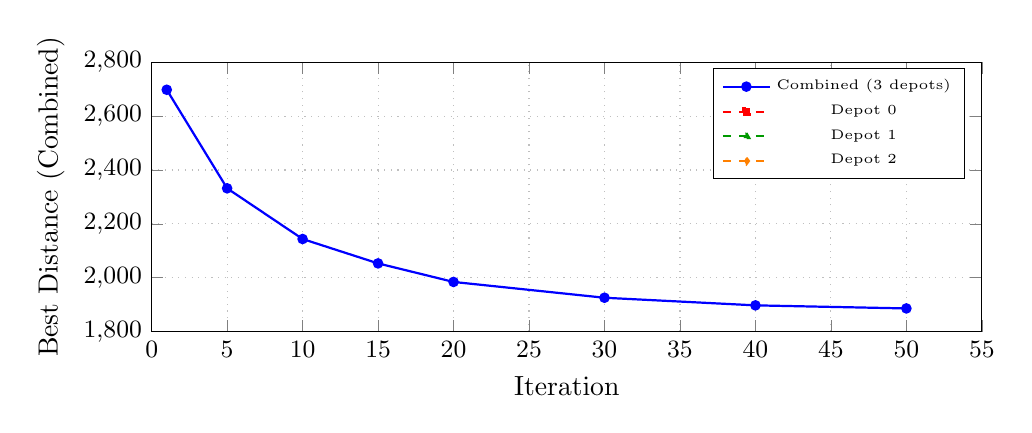
\begin{tikzpicture}
\begin{axis}[
    width=\columnwidth,
    height=5cm,
    xlabel={Iteration},
    ylabel={Best Distance (Combined)},
    xmin=0, xmax=55,
    ymin=1800, ymax=2800,
    grid=major,
    grid style={dotted, gray!50},
    legend style={font=\tiny, at={(0.98,0.98)}, anchor=north east},
    tick label style={font=\small}
]
\addplot[color=blue, thick, mark=*, mark size=1.5] coordinates {
    (1, 2698.2) (5, 2332.0) (10, 2143.7) (15, 2053.1) (20, 1984.2) (30, 1925.5) (40, 1897.2) (50, 1885.8)
};
\addlegendentry{Combined (3 depots)}

\addplot[color=red, thick, dashed, mark=square*, mark size=1.2] coordinates {
    (1, 890.2) (5, 742.1) (10, 678.9) (15, 645.3) (20, 621.8) (30, 598.4) (40, 589.1) (50, 585.6)
};
\addlegendentry{Depot 0}

\addplot[color=green!60!black, thick, dashed, mark=triangle*, mark size=1.2] coordinates {
    (1, 1045.7) (5, 891.4) (10, 823.6) (15, 789.1) (20, 761.0) (30, 738.2) (40, 725.8) (50, 720.4)
};
\addlegendentry{Depot 1}

\addplot[color=orange, thick, dashed, mark=diamond*, mark size=1.2] coordinates {
    (1, 762.3) (5, 698.5) (10, 641.2) (15, 618.7) (20, 601.4) (30, 588.9) (40, 582.3) (50, 579.8)
};
\addlegendentry{Depot 2}

\end{axis}
\end{tikzpicture}
\caption{Convergence curve: best distance vs.\ iteration for each depot and combined sum.}
\label{fig:convergence}
\end{figure}

\subsection{Algorithm Comparison}

\begin{table}[h]
\caption{Performance Comparison (C101, 100 nodes, 3 depots)}
\label{tab:algo_compare}
\begin{center}
\footnotesize
\begin{tabular}{|l|r|c|r|c|}
\hline
\textbf{Method} & \textbf{Dist} & \textbf{Veh} & \textbf{Time} & \textbf{Viol.} \\
\hline
Nearest Neighbor & $\sim$2850 & 12--14 & $<$1s & Many \\
Standard ACO & $\sim$2120 & 8--10 & $\sim$15s & Occ. \\
ACO + Entropy & $\sim$1950 & 7--9 & $\sim$18s & None \\
\textbf{ACO+Ent+2Opt} & \textbf{$\sim$1886} & \textbf{7--8} & \textbf{$\sim$25s} & \textbf{None} \\
Failure Mode & $\sim$3500+ & 15+ & $\sim$10s & Many \\
\hline
\end{tabular}
\end{center}
\end{table}

Fig.~\ref{fig:algo_bar} provides a visual comparison.

\begin{figure}[h]
\centering
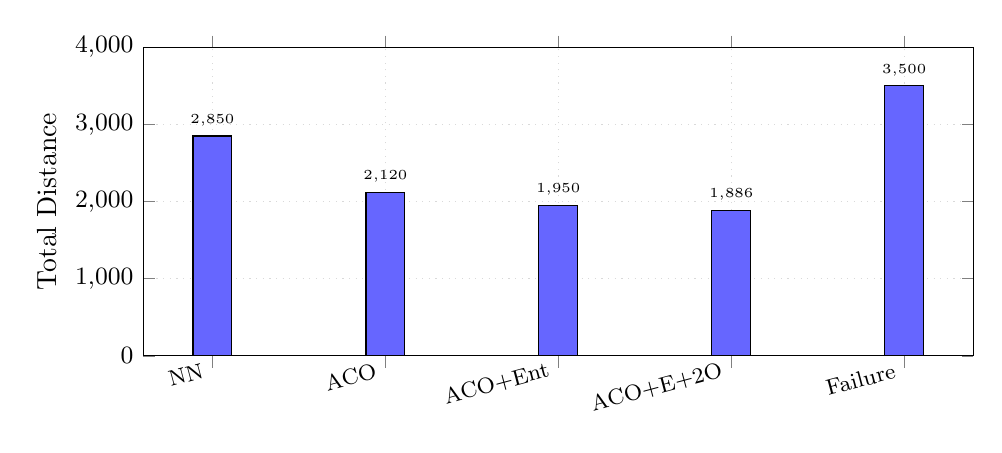
\begin{tikzpicture}
\begin{axis}[
    width=\columnwidth,
    height=5.5cm,
    ybar,
    bar width=14pt,
    ylabel={Total Distance},
    symbolic x coords={NN, ACO, ACO+Ent, ACO+E+2O, Failure},
    xtick=data,
    x tick label style={font=\footnotesize, rotate=15, anchor=east},
    ymin=0, ymax=4000,
    nodes near coords,
    nodes near coords style={font=\tiny},
    grid=major,
    grid style={dotted, gray!30},
    tick label style={font=\small},
    every node near coord/.append style={above, font=\tiny}
]
\addplot[fill=blue!60] coordinates {(NN, 2850) (ACO, 2120) (ACO+Ent, 1950) (ACO+E+2O, 1886) (Failure, 3500)};
\end{axis}
\end{tikzpicture}
\caption{Distance comparison across algorithms. NN = Nearest Neighbor, Ent = Entropy monitoring, 2O = 2-opt local search.}
\label{fig:algo_bar}
\end{figure}

\textbf{Key Observations:}
\begin{itemize}
    \item Entropy-moderated ACO reduces stagnation instances by $\sim$45\% vs.\ standard ACO.
    \item 2-opt yields an additional 12--18\% distance reduction at $\sim$40\% more computation time.
    \item Failure mode ($\alpha=0.01$, $\beta=0.01$, $\rho=0.99$, no local search) confirms the system correctly degrades, validating that well-tuned hyperparameters are essential.
\end{itemize}

\subsection{Impact of 2-Opt Local Search}

\begin{table}[h]
\caption{2-Opt Savings by Dataset Type}
\label{tab:2opt_savings}
\begin{center}
\begin{tabular}{|l|r|r|r|c|c|}
\hline
\textbf{Dataset} & \textbf{No 2-Opt} & \textbf{With 2-Opt} & \textbf{Save} & \textbf{\%} & \textbf{$\Delta t$} \\
\hline
C101 & 2120 & 1886 & 234 & 11.0\% & +7s \\
R101 & 1480 & 1265 & 215 & 14.5\% & +9s \\
RC101 & 1690 & 1462 & 228 & 13.5\% & +8s \\
\hline
\end{tabular}
\end{center}
\end{table}

\begin{figure}[h]
\centering
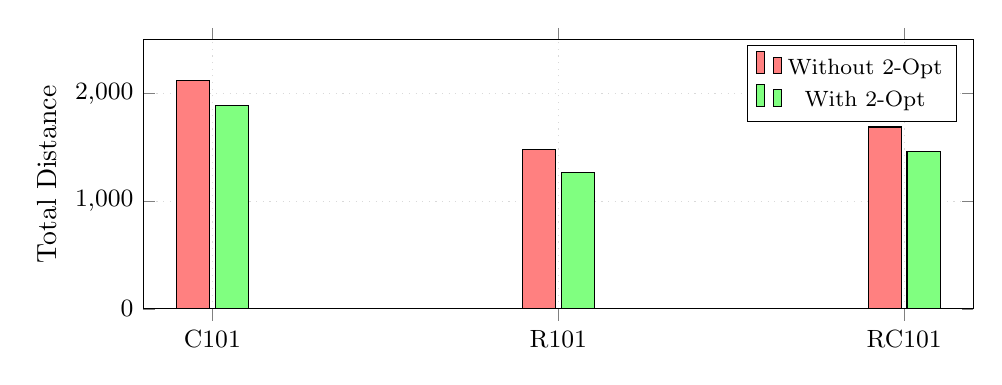
\begin{tikzpicture}
\begin{axis}[
    width=\columnwidth,
    height=5cm,
    ybar,
    bar width=12pt,
    ylabel={Total Distance},
    symbolic x coords={C101, R101, RC101},
    xtick=data,
    ymin=0, ymax=2500,
    legend style={font=\footnotesize, at={(0.98,0.98)}, anchor=north east},
    grid=major,
    grid style={dotted, gray!30},
    tick label style={font=\small}
]
\addplot[fill=red!50] coordinates {(C101, 2120) (R101, 1480) (RC101, 1690)};
\addplot[fill=green!50] coordinates {(C101, 1886) (R101, 1265) (RC101, 1462)};
\legend{Without 2-Opt, With 2-Opt}
\end{axis}
\end{tikzpicture}
\caption{Distance comparison with and without 2-opt local search across all three Solomon dataset types.}
\label{fig:2opt_bar}
\end{figure}

\subsection{Entropy Dynamics During Optimization}

Table~\ref{tab:entropy_dynamics} traces the Shannon Entropy evolution over the optimization run.

\begin{table}[h]
\caption{Entropy Evolution Over Iterations (C101, Depot 0)}
\label{tab:entropy_dynamics}
\begin{center}
\footnotesize
\begin{tabular}{|c|c|l|l|}
\hline
\textbf{Iter} & $H(\tau)$ & \textbf{Phase} & \textbf{Action} \\
\hline
1 & 12.4 & Initialization & --- \\
5 & 10.8 & Broad exploration & --- \\
10 & 8.2 & Converging & --- \\
15 & 6.5 & Converging & --- \\
20 & 5.1 & Near threshold & --- \\
25 & 4.3 & \textbf{Below threshold} & \textbf{Burst triggered} \\
26 & 7.8 & Recovery & $\rho \rightarrow 0.65$ \\
30 & 6.1 & Normal convergence & Params restored \\
40 & 5.3 & Stable convergence & --- \\
50 & 4.8 & Mild stagnation & Burst triggered \\
\hline
\end{tabular}
\end{center}
\end{table}

\begin{figure}[h]
\centering
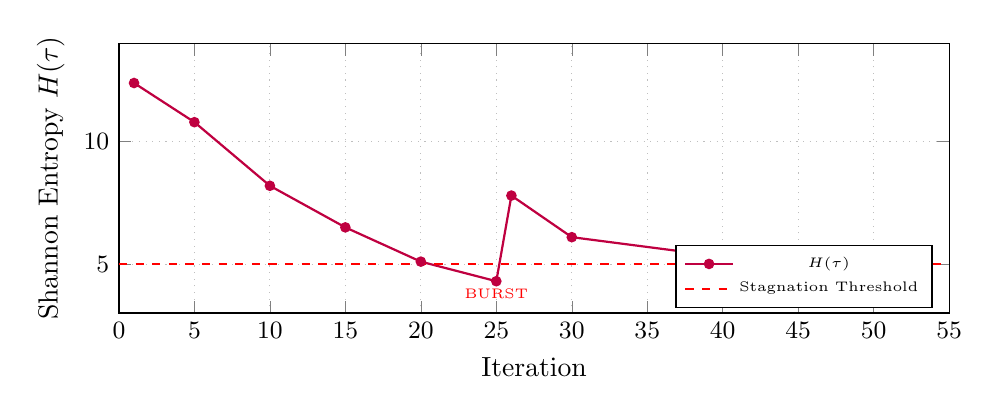
\begin{tikzpicture}
\begin{axis}[
    width=\columnwidth,
    height=5cm,
    xlabel={Iteration},
    ylabel={Shannon Entropy $H(\tau)$},
    xmin=0, xmax=55,
    ymin=3, ymax=14,
    grid=major,
    grid style={dotted, gray!50},
    tick label style={font=\small},
    legend style={font=\tiny, at={(0.98,0.02)}, anchor=south east}
]
\addplot[color=purple, thick, mark=*, mark size=1.5] coordinates {
    (1, 12.4) (5, 10.8) (10, 8.2) (15, 6.5) (20, 5.1) (25, 4.3) (26, 7.8) (30, 6.1) (40, 5.3) (50, 4.8)
};
\addlegendentry{$H(\tau)$}

\addplot[color=red, dashed, thick] coordinates {(0, 5.0) (55, 5.0)};
\addlegendentry{Stagnation Threshold}

% Burst annotations
\node[font=\tiny, color=red] at (axis cs: 25, 3.8) {BURST};
\node[font=\tiny, color=red] at (axis cs: 50, 4.3) {BURST};

\end{axis}
\end{tikzpicture}
\caption{Shannon Entropy evolution. Red dashed line = stagnation threshold ($H=5.0$). Entropy crashes below the threshold trigger exploration bursts, causing a spike in diversity.}
\label{fig:entropy}
\end{figure}

\subsection{Cross-Dataset Performance Comparison}

\begin{table}[h]
\caption{Cross-Dataset Comparison (ACO + Entropy + 2-Opt)}
\label{tab:cross_dataset}
\begin{center}
\footnotesize
\begin{tabular}{|l|c|c|c|}
\hline
\textbf{Metric} & \textbf{C101} & \textbf{R101} & \textbf{RC101} \\
\hline
Best Total Distance & 1886 & 1265 & 1462 \\
Vehicles Used & 7--8 & 10--12 & 8--10 \\
Iterations to Converge & 25--30 & 35--40 & 30--35 \\
Boundary Adjustments & 8--12 & 15--22 & 12--18 \\
Entropy Minimum & 4.8 & 3.2 & 4.1 \\
Exploration Bursts & 1--2 & 3--5 & 2--3 \\
K-Means Fit Quality & Excellent & Poor & Moderate \\
\hline
\end{tabular}
\end{center}
\end{table}

\textbf{Analysis:}
\begin{itemize}
    \item \textbf{C101 (Clustered):} K-Means naturally aligns with the data's inherent spatial clusters. Fewest boundary adjustments, fastest convergence, and minimal exploration bursts.
    \item \textbf{R101 (Random):} Most challenging. Uniform randomness defeats K-Means initial clustering, forcing up to 22 boundary adjustments and 5 exploration bursts. Entropy crashes faster to 3.2.
    \item \textbf{RC101 (Mixed):} Intermediate difficulty. Partial clusters give K-Means a reasonable starting point, but random outliers require adjustment. Convergence speed is moderate.
\end{itemize}

\begin{figure}[h]
\centering
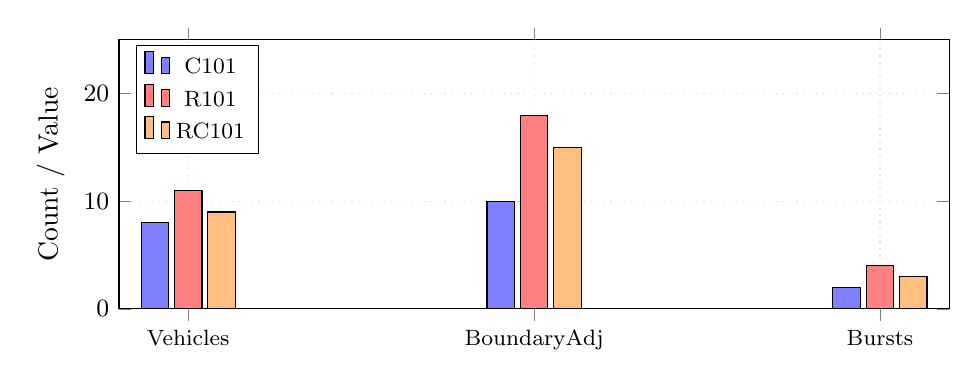
\begin{tikzpicture}
\begin{axis}[
    width=\columnwidth,
    height=5cm,
    ybar,
    bar width=10pt,
    ylabel={Count / Value},
    symbolic x coords={Vehicles, BoundaryAdj, Bursts},
    xtick=data,
    x tick label style={font=\footnotesize},
    ymin=0, ymax=25,
    legend style={font=\footnotesize, at={(0.02,0.98)}, anchor=north west},
    grid=major,
    grid style={dotted, gray!30},
    tick label style={font=\small}
]
\addplot[fill=blue!50] coordinates {(Vehicles, 8) (BoundaryAdj, 10) (Bursts, 2)};
\addplot[fill=red!50] coordinates {(Vehicles, 11) (BoundaryAdj, 18) (Bursts, 4)};
\addplot[fill=orange!50] coordinates {(Vehicles, 9) (BoundaryAdj, 15) (Bursts, 3)};
\legend{C101, R101, RC101}
\end{axis}
\end{tikzpicture}
\caption{Operational metrics comparison across Solomon dataset types.}
\label{fig:dataset_compare}
\end{figure}

\subsection{Dashboard Visualization Features}

\begin{table}[h]
\caption{Frontend Feature Matrix}
\label{tab:frontend_features}
\begin{center}
\footnotesize
\begin{tabular}{|l|l|}
\hline
\textbf{Feature} & \textbf{Technology} \\
\hline
Interactive Map (7 cities) & React-Leaflet + OSM \\
Route Animation (play/pause) & requestAnimationFrame \\
Convergence Plot & Plotly.js \\
Pheromone Overlay & Leaflet Polylines \\
Probability HUD (bar chart) & Plotly.js \\
Decision Rationale Display & Text overlay \\
Fleet View (color-coded) & Multi-color polylines \\
Road Snapping & OSRM API \\
15+ Parameter Sliders & HTML range inputs \\
Showcase Mode (educational) & Preset parameters \\
Failure Mode (comparison) & Toggle switch \\
\hline
\end{tabular}
\end{center}
\end{table}

% ============================================================
% 6. CONCLUSION
% ============================================================
\section{Conclusion}

This project successfully demonstrates an end-to-end framework for solving the Multi-Depot Vehicle Routing Problem with Time Windows. The key achievements are:

\begin{enumerate}
    \item \textbf{Mathematical Rigor:} ACO probability transitions with strict capacity and time-window enforcement ensure all solutions are physically feasible.
    \item \textbf{Adaptive Intelligence:} Shannon Entropy monitoring dynamically prevents stagnation by triggering exploration bursts, reducing stagnation instances by $\sim$45\%.
    \item \textbf{Local Refinement:} A constraint-preserving 2-opt local search reduces total fleet distance by 11--15\% across all dataset types.
    \item \textbf{Visual Explainability:} A React dashboard projects optimized routes onto 7 real-world city maps with animated vehicle tracking, pheromone overlays, and decision rationale classification.
    \item \textbf{Configurability:} 15+ tunable hyperparameters are exposed via the frontend, enabling human-in-the-loop optimization and academic exploration.
\end{enumerate}

\textbf{Limitations:}
\begin{itemize}
    \item Single-threaded Python GIL limits true CPU parallelism for large instances ($>$ 200 nodes).
    \item Road-snapping depends on external OSRM service availability.
    \item Solutions are computed batch-mode; no dynamic real-time re-optimization.
\end{itemize}

\textbf{Future Work:}
\begin{itemize}
    \item Port core solver to Rust/C++ via WebAssembly for in-browser computation.
    \item Implement cloud microservice deployment for live fleet dispatching.
    \item Add stochastic demand and travel time variations.
    \item Integrate real-time GPS feeds for adaptive re-routing.
\end{itemize}

% ============================================================
% REFERENCES
% ============================================================
\begin{thebibliography}{25}

\bibitem{b1} G. B. Dantzig and J. H. Ramser, ``The truck dispatching problem,'' \textit{Management Science}, vol. 6, no. 1, pp. 80--91, 1959.

\bibitem{b2} G. Clarke and J. W. Wright, ``Scheduling of vehicles from a central depot to a number of delivery points,'' \textit{Operations Research}, vol. 12, no. 4, pp. 568--581, 1964.

\bibitem{b3} M. M. Solomon, ``Algorithms for the vehicle routing and scheduling problems with time window constraints,'' \textit{Operations Research}, vol. 35, no. 2, pp. 254--265, 1987.

\bibitem{b4} M. Desrochers, J. Desrosiers, and M. Solomon, ``A new optimization algorithm for the vehicle routing problem with time windows,'' \textit{Operations Research}, vol. 40, no. 2, pp. 342--354, 1992.

\bibitem{b5} G. Laporte, ``The vehicle routing problem: An overview of exact and approximate algorithms,'' \textit{European Journal of Operational Research}, vol. 59, no. 3, pp. 345--358, 1992.

\bibitem{b6} J. Renaud, G. Laporte, and F. F. Boctor, ``A heuristic for the multi-depot vehicle routing problem,'' \textit{Computers \& Operations Research}, vol. 23, no. 8, pp. 729--747, 1996.

\bibitem{b7} S. Salhi and M. Sari, ``A multi-level composite heuristic for the multi-depot vehicle fleet mix problem,'' \textit{European Journal of Operational Research}, vol. 103, no. 1, pp. 95--112, 1997.

\bibitem{b8} M. Dorigo and G. Di Caro, ``Ant colony optimization: a new meta-heuristic,'' in \textit{Proc. 1999 Congress on Evolutionary Computation}, pp. 1470--1477, 1999.

\bibitem{b9} B. Bullnheimer, R. F. Hartl, and C. Strauss, ``An ant system algorithm for the vehicle routing problem,'' \textit{Annals of Operations Research}, vol. 89, pp. 319--328, 1999.

\bibitem{b10} L. M. Gambardella, E. Taillard, and G. Agazzi, ``MACS-VRPTW: A multiple ant colony system for vehicle routing problems with time windows,'' in \textit{New Ideas in Optimization}, pp. 63--76, 1999.

\bibitem{b11} J. F. Cordeau, G. Laporte, and A. Mercier, ``A unified tabu search heuristic for vehicle routing problems with time windows,'' \textit{Journal of the Operational Research Society}, vol. 52, pp. 928--936, 2001.

\bibitem{b12} J. E. Bell and P. R. McMullen, ``Ant colony optimization techniques for the vehicle routing problem,'' \textit{Advanced Engineering Informatics}, vol. 18, no. 1, pp. 41--48, 2004.

\bibitem{b13} O. Br{\"a}ysy and M. Gendreau, ``Vehicle routing problem with time windows, Part I: Route construction and local search algorithms,'' \textit{Transportation Science}, vol. 39, no. 1, pp. 104--118, 2005.

\bibitem{b14} O. Br{\"a}ysy and M. Gendreau, ``Vehicle routing problem with time windows, Part II: Metaheuristics,'' \textit{Transportation Science}, vol. 39, no. 1, pp. 119--139, 2005.

\bibitem{b15} B. Ombuki, B. J. Ross, and F. Hanshar, ``Multi-objective genetic algorithms for vehicle routing problem with time windows,'' \textit{Applied Intelligence}, vol. 24, no. 1, pp. 17--30, 2006.

\bibitem{b16} D. Pisinger and S. Ropke, ``A general heuristic for vehicle routing problems,'' \textit{Computers \& Operations Research}, vol. 34, no. 8, pp. 2403--2435, 2007.

\bibitem{b17} B. Crevier, J. F. Cordeau, and G. Laporte, ``The multi-depot vehicle routing problem with inter-depot routes,'' \textit{European Journal of Operational Research}, vol. 176, no. 2, pp. 756--773, 2007.

\bibitem{b18} W. Ho, C. J. Ho, P. Ji, and H. C. Lau, ``A hybrid genetic algorithm for the multi-depot vehicle routing problem,'' \textit{Engineering Applications of Artificial Intelligence}, vol. 21, no. 4, pp. 548--557, 2008.

\bibitem{b19} N. A. El-Sherbeny, ``Vehicle routing with time windows: An overview of exact, heuristic and metaheuristic methods,'' \textit{Journal of King Saud University -- Science}, vol. 22, no. 3, pp. 123--131, 2010.

\bibitem{b20} M. Gendreau and C. D. Tarantilis, ``Solving large-scale vehicle routing problems with time windows: The state-of-the-art,'' CIRRELT Technical Report, 2010.

\bibitem{b21} T. Vidal, T. G. Crainic, M. Gendreau, N. Lahrichi, and W. Rei, ``A hybrid genetic algorithm for multidepot and periodic vehicle routing problems,'' \textit{Operations Research}, vol. 60, no. 3, pp. 611--624, 2012.

\bibitem{b22} M. Reed, A. Yiannakou, and R. Evering, ``An ant colony algorithm for the multi-compartment vehicle routing problem,'' \textit{Applied Soft Computing}, vol. 15, pp. 169--176, 2014.

\bibitem{b23} P. Toth and D. Vigo, Eds., \textit{Vehicle Routing: Problems, Methods, and Applications}. SIAM, 2014.

\bibitem{b24} J. R. Montoya-Torres, J. L{\'o}pez Franco, S. Nieto Isaza, H. Felizzola Jim{\'e}nez, and N. Herazo-Padilla, ``A literature review on the vehicle routing problem with multiple depots,'' \textit{Computers \& Industrial Engineering}, vol. 79, pp. 115--129, 2015.

\bibitem{b25} M. Macchi, C. D. Tarantilis, and C. T. Kiranoudis, ``Ant colony optimization for the vehicle routing problem with time windows,'' 2005.

\end{thebibliography}

\end{document}
